\documentclass{article}
\usepackage[utf8]{inputenc}
% >>>> DO NOT EDIT THIS FILE
% If you *must* add or change a macro, please email fkoh@caltech.edu

%=================================================
% Basics
%=================================================

\usepackage{fixltx2e} % Makes \( \) equation style robust, among other
                      % things. Must be the first package.


% Makes ligatured fonts searchable and copyable in pdf readers
\usepackage{cmap} % Load before fontenc
\usepackage[spanish]{babel}

% Always include these font encodings in your document
% unless you have a very good reason.
\usepackage[T1]{fontenc}
\usepackage[utf8]{inputenc}

\usepackage{verbatim}

%=====================================
% Look & feel
%=====================================

% Allows for manual space setting
\usepackage{setspace}

%=============
% Fonts
%=============

\usepackage{lmodern} % Improved version of computer modern
\usepackage[scale=0.88]{tgheros} % Helvetica clone for sans serif font


\newcommand\hmmax{2} % Default is 3.
\newcommand\bmmax{2} % Default is 4.

\usepackage{bm} % boldmath must be called after the package
\providecommand{\mathbold}[1]{\bm{#1}}

%=============
% AMS Packages and fonts
%=============
\usepackage{amsmath,amsbsy,amsgen,amscd,amsthm,amsfonts,amssymb}

%=============
% Margins and paper size
%=============
\usepackage[centering,top=1.5in,bottom=1.2in,left=1.4in,right=1.4in]{geometry}

%=============
% Title setup
%=============
\usepackage{titling}
%\usepackage{nopageno}
\setlength{\droptitle}{-7.5em}

\pretitle{\noindent\rule{0.85\linewidth}{0.2mm}\par%
  \begin{raggedright}\LARGE\sffamily}
\posttitle{\par\end{raggedright}%
\noindent%
\rule{0.85\linewidth}{0.5mm}\par}

\preauthor{\noindent\vspace{0.5em}%
  \sffamily\begin{tabular}[t]{ll}}
  \postauthor{\end{tabular}\par\thispagestyle{plain}}

\predate{\noindent%
  \small\sffamily\itshape\begin{tabular}[t]{l}%
    EST-25134, Primavera 2021 \\ %
    Profesor: Dr.\ Alfredo Garbuno Iñigo \\ %
  }
  \postdate{
  \end{tabular}\par}

%=============
% Section headings
%=============
\usepackage[sf,bf,compact]{titlesec}

%=============
% Tables and lists
%=============
\usepackage{booktabs,longtable,tabu} % Nice tables
\setlength{\tabulinesep}{1mm}
\usepackage[font=small,margin=10pt,labelfont={sf,bf},labelsep={space}]{caption}


\usepackage{enumitem}
\setitemize{itemsep=0pt}
\setenumerate{itemsep=0pt}
\setlist{labelindent=\parindent,%  % Recommended by enumitem package
  font=\sffamily}


%=============
% Hyperlink colors
%=============
\usepackage[usenames,dvipsnames]{xcolor}
\definecolor{dark-gray}{gray}{0.3}
\definecolor{dkgray}{rgb}{.4,.4,.4}
\definecolor{dkblue}{rgb}{0,0,.5}
\definecolor{medblue}{rgb}{0,0,.75}
\definecolor{rust}{rgb}{0.5,0.1,0.1}

\usepackage{url}
\usepackage[colorlinks=true]{hyperref}
\hypersetup{linkcolor=dkblue}
\hypersetup{citecolor=rust}
\hypersetup{urlcolor=rust}
\usepackage[spanish, capitalise]{cleveref}
\usepackage{autonum}
%=============
% Microtype
%=============
\usepackage[final]{microtype}

%=============
% Theorems, etc.
%=============
\newtheoremstyle{myThm} % name
    {\topsep}                    % Space above
    {\topsep}                    % Space below
    {\itshape}                   % Body font
    {}                           % Indent amount
    {\sffamily\bfseries}                   % Theorem head font
    {.}                          % Punctuation after theorem head
    {.5em}                       % Space after theorem head
    {}  % Theorem head spec (can be left empty, meaning ‘normal’)

\newtheoremstyle{myRem} % name
    {\topsep}                    % Space above
    {\topsep}                    % Space below
    {}                   % Body font
    {}                           % Indent amount
    {\sffamily}                   % Theorem head font
    {.}                          % Punctuation after theorem head
    {.5em}                       % Space after theorem head
    {}  % Theorem head spec (can be left empty, meaning ‘normal’)

\newtheoremstyle{myDef} % name
    {\topsep}                    % Space above
    {\topsep}                    % Space below
    {}                   % Body font
    {}                           % Indent amount
    {\sffamily\bfseries}                   % Theorem head font
    {.}                          % Punctuation after theorem head
    {.5em}                       % Space after theorem head
    {}  % Theorem head spec (can be left empty, meaning ‘normal’)

\theoremstyle{myThm}
\newtheorem{theorem}{Teorema}[section]
\newtheorem{lemma}[theorem]{Lemma}
\newtheorem{proposition}[theorem]{Proposition}
\newtheorem{corollary}[theorem]{Corollary}
\newtheorem{fact}[theorem]{Fact}

\theoremstyle{myRem}
\newtheorem{remark}[theorem]{Remark}

\theoremstyle{myDef}
\newtheorem{definition}[theorem]{Definition}
\newtheorem{example}[theorem]{Example}

%=====================
% Header
%=====================
\usepackage{fancyhdr}
\usepackage{nopageno} % Gets rid of page number at the bottom
\fancyhf{} % Clear header style
\renewcommand{\headrulewidth}{0.5pt} % remove the header rule
\pagestyle{fancy}
\fancyhead[LE,RO]{\textsf{\small \thepage}}

\setlength{\headheight}{14pt}
%=====================
% Fix delimiters
%=====================

% Fixes \left and \right spacing issues. See discussion at
% http://tex.stackexchange.com/questions/2607/spacing-around-left-and-right
\let\originalleft\left
\let\originalright\right
\renewcommand{\left}{\mathopen{}\mathclose\bgroup\originalleft}
\renewcommand{\right}{\aftergroup\egroup\originalright}

%=================================================
% Math macros
%=================================================

%=============
% Generalities
%=============
\usepackage{mathtools}
\mathtoolsset{centercolon}  % Makes := typeset correctly for definitions

%%% Equation numbering
%\numberwithin{equation}{section}

%%% Annotations
\newcommand{\notate}[1]{\textcolor{red}{\textbf{[#1]}}}

%==============
% Symbols
%==============
\let\oldphi\phi
\let\oldeps\epsilon
\let\oldemptyset\emptyset
\let\emptyset\varnothing

\renewcommand{\phi}{\varphi}
\renewcommand{\epsilon}{\varepsilon}
\newcommand{\eps}{\varepsilon}
\newcommand{\cl}{\mathrm{cl}}
\newcommand{\wto}{\rightharpoonup}
\newcommand{\wsto}{\overset{\ast}{\rightharpoonup}}
\newcommand{\wwto}{\overset{w}{\to}}
\newcommand{\wwsto}{\overset{w*}{\to}}

%==============
% Constants
%==============

% Set constants upright
\newcommand{\cnst}[1]{\mathrm{#1}}
\newcommand{\econst}{\mathrm{e}}
\newcommand{\rd}{\mathrm{d}}
\newcommand{\dist}{\mathrm{dist}}

\newcommand{\zerovct}{\vct{0}} % Zero vector
\newcommand{\Id}{\mathbf{I}} % Identity matrix
\newcommand{\onemtx}{\bm{1}}
\newcommand{\zeromtx}{\bm{0}}

%==============
% Sets
%==============
\providecommand{\mathbbm}{\mathbb} % In case we don't load bbm

% Reals, complex, naturals, integers, field
\newcommand{\R}{\mathbbm{R}}
\newcommand{\C}{\mathbbm{C}}
\newcommand{\N}{\mathbbm{N}}
\newcommand{\Z}{\mathbbm{Z}}
\newcommand{\F}{\mathbbm{F}}

%==============
% Probability
%==============
\newcommand{\Prob}{\operatorname{\mathbbm{P}}}
\newcommand{\Expect}{\operatorname{\mathbb{E}}}
\newcommand{\D}{\operatorname{\mathcal{D}}}

%==============
% Vectors and matrices
%==============
\newcommand{\vct}[1]{\mathbold{#1}}
\newcommand{\mtx}[1]{\mathbold{#1}}

%=============
% Operators
%=============
\newcommand{\B}{\mathcal{B}}
\newcommand{\op}[1]{\mathbold{#1}}

\title{Clase 8: Compromiso entre sesgo y varianza}
\author{Responsable: Santiago Ruiz Velasco Fernández}
\date{Febrero 9, 2021}

\begin{document}

\maketitle

\section{Introducción}
Como hemos estudiado a través de los modelos lineales, para contrarrestar el riesgo de sobreajuste, una alternativa es utilizar una familia de hipótesis $\mathcal{H}$ más restringida, asegurando que se encuentre todo nuestro conocimiento previo. Sin embargo, este conocimiento previo puede causar un sesgo en el aprendizaje. Ahora, para evitar que nuestro aprendizaje esté sesgado, lo que esperaríamos es que nuestra familia de hipótesis no posea sesgo y que sea universalmente aplicable.
\vspace{0.3cm}

Recordemos que una tarea de aprendizaje se define a través de la distribución $D$ definida en $\mathcal{X}$x$\mathcal{Y}$, con $\mathcal{X}$ conjunto de atributos y $\mathcal{Y}$ variables objetivo donde buscamos alguna h: $\mathcal{X}\xrightarrow{}\mathcal{Y}$ de tal forma que el error de generalización o el riesgo teórico $L_D(h)$ sea mínimo. 
\vspace{0.3cm}

¿Existe algún algoritmo de aprendizaje $A$ y un conjunto de entrenamiento $S$ con $|S| = m$ tal que para toda distribución $D$, si A recibe las $m$ observaciones independientes e idénticamente distribuidas en $D$, entonces con alta probabilidad lograremos encontrar esa hipótesis h: $\mathcal{X}\xrightarrow{}\mathcal{Y}$ tal que el error de generalización $L_D(h)$ \ll $\epsilon$? Si se puede contestar afirmativamente esta pregunta, entonces sabremos que existe la familia de hipótesis $\mathcal{H}$ insesgada y universalmente aplicable  


\section{Teorema: No Free Lunch (NFL)}
\subsection{Explicación}
El nombre de este teorema nos da a entender un poco mejor el contexto de un problema de clasificación con un ejemplo simple: así como no es posible tener un almuerzo que sea completamente gratuito, no existe ninguna distribución donde nuestra mejor hipótesis candidata esté libre de fallos, es decir, para alguna distribución, no importa que tengamos a un modelo candidato que nosotros consideremos el "mejor" teóricamente, este va a fallar. Por este teorema podemos concluir que no existe una familia de hipótesis $\mathcal{H}$ que sea universalmente aplicable.
\subsection{Descomposición del error cometido por ERM}
Esta descomposición se analizará en dos partes:
\begin{enumerate}
    \item Calidad de $\mathcal{H}$: Habla del posible sesgo que pueda presentar el aprendizaje.
    \item Riesgo de sobreajuste: Habla sobre la varianza que presenta el aprendizaje al observar distintos conjuntos de datos.
\end{enumerate}
La idea principal es que dependiendo del modelo que nosotros utilicemos, el error cometido por el ERM presentará diferentes problemas:
\vspace{0.3cm}

Si nuestro modelo es altamente complejo, este emitirá un aprendizaje con menor sesgo, pero con una mayor varianza. Por otro lado, con un modelo simple, como una regresión lineal, presentará una varianza pequeña, pero tendrá mucho sesgo.
\vspace{0.5cm}
\subsection{Enunciación del Teorema y Demostración}
\begin{center}
    \begin{theorem}[No Free Lunch (NFL)]
    Sea $A$ un algoritmo de aprendizaje con dominio finito $\mathcal{X}$ y conjunto objetivo $\mathcal{Y}$=\{0,1\}. Sea m un entero tal que m < $\frac{|\mathcal{X}|}{2}$. Entonces existe una distribución con soporte $\mathcal{X}$x$\mathcal{Y}$ tal que
    \begin{enumerate}
        \item Existe una función de etiquetado f: $\mathcal{X}\xrightarrow{}\mathcal{Y}$ con un error de generalización nulo, es decir, $L_D(f)=0$
        \item Con probabilidad mayor o igual a $\frac{1}{7}$ sobre posibles realizaciones de nuestros conjuntos de entrenamiento S \sim $D^{m}$, tenemos que el riesgo empírico de realizar el algoritmo de aprendizaje A a S no puede disminuir más de $\frac{1}{8}$, es decir: 
        \begin{center}
            $\mathbb{P}_{S \sim D^{m}}(L_D(A(S)) \ge \frac{1}{8}) \ge \frac{1}{7}$
        \end{center}
    \end{enumerate}
     
    \end{theorem}
\end{center}
En pocas palabras, aunque encontremos una hipótesis f "perfecta", hay una distribución donde nuestra clasificación resulta no ser tan baja como se esperaba. La intuición de la demostración que veremos a continuación es que cualquier algoritmo que vea la mitad de algún subconjunto de $\mathcal{X}$ no va a tener información suficiente sobre el resto. Esto va a llevar a que exista una función de etiquetado que contradiga las etiquetas ya aprendidas
    \begin{proof}
    Sea $C \subset \mathcal{X}$  con |C|=2m. 
    
    \vspace{0.3cm}
    Además, sea T el conjunto que contiene a todas las posibles funciones f: C$\xrightarrow{}\mathcal{Y}$. Por cómo está definido, |T|=$2^{2m}$ y T=$\{f_1, ..., f_T\}$.
    
    \vspace{0.3cm}
    Sea $D_i$ una distribución que actúa sobre Cx$\mathcal{Y}$ tal que con una observación \{x,y\}, tenemos que:
    \begin{center}
        $D_i(\{x,y\})$=
        \begin{cases}
            \text{$\frac{1}{|C|}$} & \quad\text{y = $f_i(x)$} \\
            \text{0} &\quad\text{en otro caso}.
        \end{cases}
    \end{center}
    Esto nos dice que $L_{D_i}(f_i)=0$
    
    \vspace{0.3cm}
    pd: Para todo A que reciba m observaciones y regrese una proyección de etiquetado A(s): C$\xrightarrow{}\mathcal{Y}$ tiene:
    \begin{center}
    \begin{center}
        $\underset{i \in \{0, ..., T\}}{\max}$ $\mathbb{E}_{S \sim D^{m}}  L_{D_i}(A(s)) \ge \frac{1}{4}$  \hspace{1.5cm} (1)
    \end{center}
    \end{center}
    \\
    Esto quiere decir que cualquier algoritmo que usemos tendrá un error mayor a $\frac{1}{4}$.
    
    \vspace{0.3cm}
    Sea k =$(2m)^m$ el número de todos los posibles conjuntos de entrenamiento, que etiquetaremos como $S_1, ...,S_k$. Esto se debe porque un conjunto de entrenamiento son realizaciones independientes de la distribución. Por ello para un conjunto de tamaño m estoy asignando 2m puntos posibles.
    
    \vspace{0.3cm}
    Si sabemos que tenemos $S_i=(x_1, ..., x_m)$, denotamos por $S^{i}_{j}$ el conjunto de muestras de $S_j$ que son etiquetadas por la i-ésima función $f_i$. Eso quiere decir que $S_j^i =\{(x_r, f_i(x_r))\}_{r=1}^m$.
    
    \vspace{0.3cm}
    Si $D_i$ es la distribución que genera los datos, podemos esperar que los conjuntos $S_1, ...,S_k$ bajo esa distribución tienen la misma probabilidad de ser seleccionados. Esto implica que la pérdida esperada usando el algoritmo de aprendizaje con los sobre S es igual al promedio de las pérdidas usando el algoritmo de aprendizaje sobre todos los conjuntos $S_j^i$ con j = 1, ..., k.
    \begin{center}
        $\mathbb{E}_{S \sim D^m}[L_{D_i}(A(S))]$ = $\frac{1}{k}\sum\limits_{j=1}^kL_{D_i}(A(S_j^i))$ \hspace{1.5cm} (2)
    \end{center}
    
    A partir de aquí, usaremos como idea principal para continuar la demostración que "máximo \ge promedio \ge mínimo"
    
    \vspace{0.3cm}
    \begin{center}
        $\underset{i \in \{0, ..., T\}}{\max}$ $\frac{1}{k}\sum\limits_{j=1}^kL_{D_i}(A(S_j^i))$ $\underset{max \ge prom}{\ge}$ $\frac{1}{T}\sum\limits_{i=1}^T\frac{1}{k}\sum\limits_{j=1}^kL_{D_i}(A(S_j^i))$ = $\frac{1}{k}\sum\limits_{j=1}^k\frac{1}{T}\sum\limits_{i=1}^TL_{D_i}(A(S_j^i))$
        $\underset{prom \ge min}{\ge}$ $\underset{j \in \{0, ..., k\}}{\min}$ $\frac{1}{T}\sum\limits_{i=1}^TL_{D_i}(A(S_j^i))$ \hspace{1.5cm} (3)
    \end{center}
    
    Considerando $j \in \{1, ..., k\}$ fija y  $S_j=(x_1, ..., x_m)$, sea $V_j=\{v_1, ..., v_p\}$ todos los objetos que no utilizamos para entrenar, es decir, $V_j = C-S_j$, donde p \ge m. Por lo tanto, para toda h: C$\xrightarrow{}\mathcal{Y}$ y para toda i, se cumple que
    \begin{center}
        $L_{D_i}(h) = \frac{1}{2m}\sum\limits_{x \in C}\mathbb{I}_{[h(x) \ne f_i(x)]} \ge \frac{1}{2m} \sum\limits_{x \in V_j}\mathbb{I}_{[h(x) \ne f_i(x)]} \ge \frac{1}{2p}\sum\limits_{x \in V_j}\mathbb{I}_{[h(x) \ne f_i(x)]}$
    \end{center}
    
    Entonces, tomando el promedio sobre las diferentes distribuciones, obtenemos que:
    \begin{center}
        $\frac{1}{T}\sum\limits_{i=1}^TL_{D_i}(A(S_j^i)) \ge \frac{1}{T}\sum\limits_{i=1}^T\frac{1}{2p}\sum\limits_{x \in V_j}\mathbb{I}_{[h(x) \ne f_i(x)]} = \frac{1}{2p}\sum\limits_{x \in V_j}\frac{1}{T}\sum\limits_{i=1}^T\mathbb{I}_{[h(x) \ne f_i(x)]}$  
        \\
        $\underset{prom \ge min}{\ge}$ $\frac{1}{2}$ $\underset{r \in \{1, ..., p\}}{\min}$ $\frac{1}{T}\sum\limits_{i=1}^T\mathbb{I}_{[h(x) \ne f_i(x)]}$ \hspace{1.5cm} (4)
    \end{center}
    
    Considerando r fija (es decir, $v_r$ fijo, que es un dato con el cual no entrenamos el algoritmo), se pueden partir las funciones $f_1, ..., f_T$ en pares donde cada par $(f_i, f_{i'})$ tiene como característica que para cualquier observación posible $c \in C$, la etiqueta $f_i(c) \ne f_{i'}(c)$ si y solo si $c=v_r$
    
    $\implies$ El conjunto de entrenamiento que $S_i = S_{i'}$
    
    $\implies$ $\mathbb{I}_{[A(S_j^i(v_r) \ne f_i(v_r)]}+\mathbb{I}_{[A(S_j^{i'}(v_r) \ne f_{i'}(v_r)]}=1$, es decir, uno lo califica mal y el otro lo califica bien.
    
    $\implies$ $\frac{1}{T}\sum\limits_{i=1}^T\mathbb{I}_{[A(S_j^i(v_r) \ne f_i(v_r)]} = \frac{1}{T}\frac{T}{2} = \frac{1}{2}$ \hspace{1.5cm} (5)
    
    \vspace{0.3}
    Esto se debe a que tenemos T términos, y al estar pareadas lo dividimos a la mitad, tomando todas las clasificaciones distintas.
    
    \vspace{0.3cm}
    
    Aplicando (5) en (4), obtenemos que:
    \begin{center}
        $\frac{1}{T}\sum\limits_{i=1}^TL_{D_i}(A(S_j^i)) \ge$ $\frac{1}{2} \underset{r \in \{1, ..., p\}}{\min}$ $\frac{1}{T}\sum\limits_{i=1}^T\mathbb{I}_{[h(x) \ne f_i(x)]}$ = $\frac{1}{2} \underset{r \in \{1, ..., p\}}{\min} \frac{1}{2}$ = $\frac{1}{4}$
    \end{center}
    
    Aplicando (4) en (3), obtenemos que:
    \begin{center}
        $\underset{i \in \{0, ..., T\}}{\max}$ $\frac{1}{k}\sum\limits_{j=1}^kL_{D_i}(A(S_j^i)) \ge \underset{j \in \{0, ..., k\}}{\min}$ $\frac{1}{T}\sum\limits_{i=1}^TL_{D_i}(A(S_j^i)) \ge \underset{j \in \{0, ..., k\}}{\min} \frac{1}{4} = \frac{1}{4}$  
    \end{center}
    Aplicando (3) en (2), obtenemos que:
    \begin{center}
        $\mathbb{E}_{S \sim D^m}[L_{D_i}(A(S))]$ = $\frac{1}{k}\sum\limits_{j=1}^kL_{D_i}(A(S_j^i))$ \\
        $\implies$ $\underset{i \in \{0, ..., T\}}{\max}$ $\mathbb{E}_{S \sim D^m}[L_{D_i}(A(S))]$ = $\underset{i \in \{0, ..., T\}}{\max}$ $\frac{1}{k}\sum\limits_{j=1}^kL_{D_i}(A(S_j^i)) \ge \frac{1}{4}$.
    \end{center}
    Revisando la aplicación de (3) en (2), podemos observar que llegamos a (1), así demostrando la primera parte.
    \vspace{0.3cm}
    
    pd: $\mathbb{E}_{S \sim D^m}[L_{D_i}(A(S))] \ge \frac{1}{4} \implies \mathbb{P}_{S \sim D^{m}}(L_D(A(S)) \ge 1/8) \ge \frac{1}{7}$
    \vspace{0.3cm}
    
    Recordemos que la desigualdad de Markov nos dice que para una variable aleatoria X donde $\mathbb{E}[X] \ge \alpha$, entonces
    \begin{center}
        $\mathbb{P}(X \ge 1-p) \ge \frac{\alpha - (1-p)}{p}$
    \end{center}
    De este resultado, como sabemos que $\mathbb{E}_{S \sim D^m}[L_{D_i}(A(S))] \ge \frac{1}{4}$, concluimos por la desigualdad de Markov que:
    \begin{center}
        $\mathbb{P}_{S \sim D^{m}}(L_D(A(S)) \ge 1 - \frac{7}{8}) \ge  \frac{\frac{1}{4}-(1-\frac{7}{8})}{\frac{7}{8}} = \frac{1}{7}$
    \end{center}
    \end{proof}
\subsection{¿Cómo relacionamos NFL con el conocimiento previo}
\begin{corollary}
Sea $\mathcal{X}$ un conjunto infinito y sea $\mathcal{H}$ = \{f:$\mathcal{X}\xrightarrow{}\{0,1\}$\}. Entonces $\mathcal{H}$ no es aprendible en el sentido PAC (probable y aproximadamente correcto).
\end{corollary}
\begin{proof}
Asumamos que $\mathbb{H}$ es aprendible en el sentido PAC. Dada $\epsilon < \frac{1}{8}$ y $\delta < \frac{1}{7}$, esto implica que existe un algoritmo A y un entero $m = m(\epsilon, \delta)$ que denota el tamaño de muestra suficiente tal que para toda función de etiquetado f:$\mathcal{X}\xrightarrow{}\{0,1\}$, el riesgo de realizabilidad $L_D(f)=0$, lo que implica que con probabilidad mayor o igual que 1-$\delta$ el algoritmo A con muestras m nos dará que:
\begin{center}
    $L_d(A(S)) \ge \epsilon$
\end{center}

Como |$\mathcal{X}| = \infty > 2m$, por el Teorema NFL tenemos que para todo algoritmo existe una distribución tal que con probabilidad mayor o igual que $\frac{1}{7} > \delta$, obtenermos que:
\begin{center}
    $L_D(A(S)) > \frac{1}{8} > \epsilon$
\end{center}
Esto nos lleva a una contradicción, que es causada por imponer que $\mathcal{H}$ es aprendible PAC. Por lo tanto, $\mathcal{H}$ no es aprendible en el sentido PAC.
\end{proof}

\section{Descomposición del Error}
Recordemos que denotamos a $h_s$ como el predictor que regresa el principio de minimización de riesgo empírico aplicado a una familia de posibilidades $\mathcal{H}$ $(ERM_{\mathcal{H}})$ El error de generalización $h_s$ se puede descomponer de la siguiente manera:
\begin{center}
    $L_D(h_s) = \epsilon_a + \epsilon_e$ \\
    $\epsilon_a$ := Error de aproximación; \hspace{2cm} $\epsilon_e$ := Error de estimación. \\
    $\epsilon_a$ = $\underset{h \in \mathcal{H}}{\min}$ $L_D{h}$; \hspace{4cm} $\epsilon_e = L_D(h_s) - \epsilon_a$.
\end{center}
$\epsilon_a$ representa el riesgo mínimo de la clase (sesgo inductivo), y $\epsilon_e$ es la diferencia entre nuestra aproximación con el método ERM y lo que hubiéramos esperado de la clase de posibilidades que estamos tomando en cuenta. De aquí tomamos en cuenta dos posibilidades:
\begin{enumerate}
    \item $\mathcal{H}$ es muy flexible, lo cual causa que $\epsilon_a$ disminuya, pero $\epsilon_e$ aumente. A esto lo conocemos como sobreajuste.
    \item $\mathcal{H}$ es muy flexible, lo cual causa que $\epsilon_a$ aumente , pero $\epsilon_e$ disminuye. A esto lo conocemos como subajuste.
\end{enumerate}
Esto lleva a que si aumentamos la flexibilidad de nuestra familia de funciones encontremos resultados poco favorables, pero si la familia es muy rígida, esto causaría que los resultados no estén bien generalizados, que hace que no sea lo suficientemente complejo.

\vspace{0.3cm}
Visto de forma más gráfica, si nuestra familia $\mathcal{H}$ es muy flexible, eso ocasionaría que intente conectar con la mayor cantidad de datos posibles, haciendo una gran cantidad de oscilaciones para llegar a esos puntos. En casos donde sea muy difícil llegar a esos resultados, donde los demás modelos indicarían que es un error de observación, una familia más ajustada lo tomaría como un caso particular. Por otro lado, si $\mathcal{H}$ es más rígida, a pesar de su utilidad para la estimación, habría un gran sesgo inductivo, que se puede ver porque no se acerca lo suficiente a los datos. En la siguiente figura se muestra un ejemplo gráfico con esta descripción para facilitar la visualización.

    \begin{figure}[h!]
      \centering
      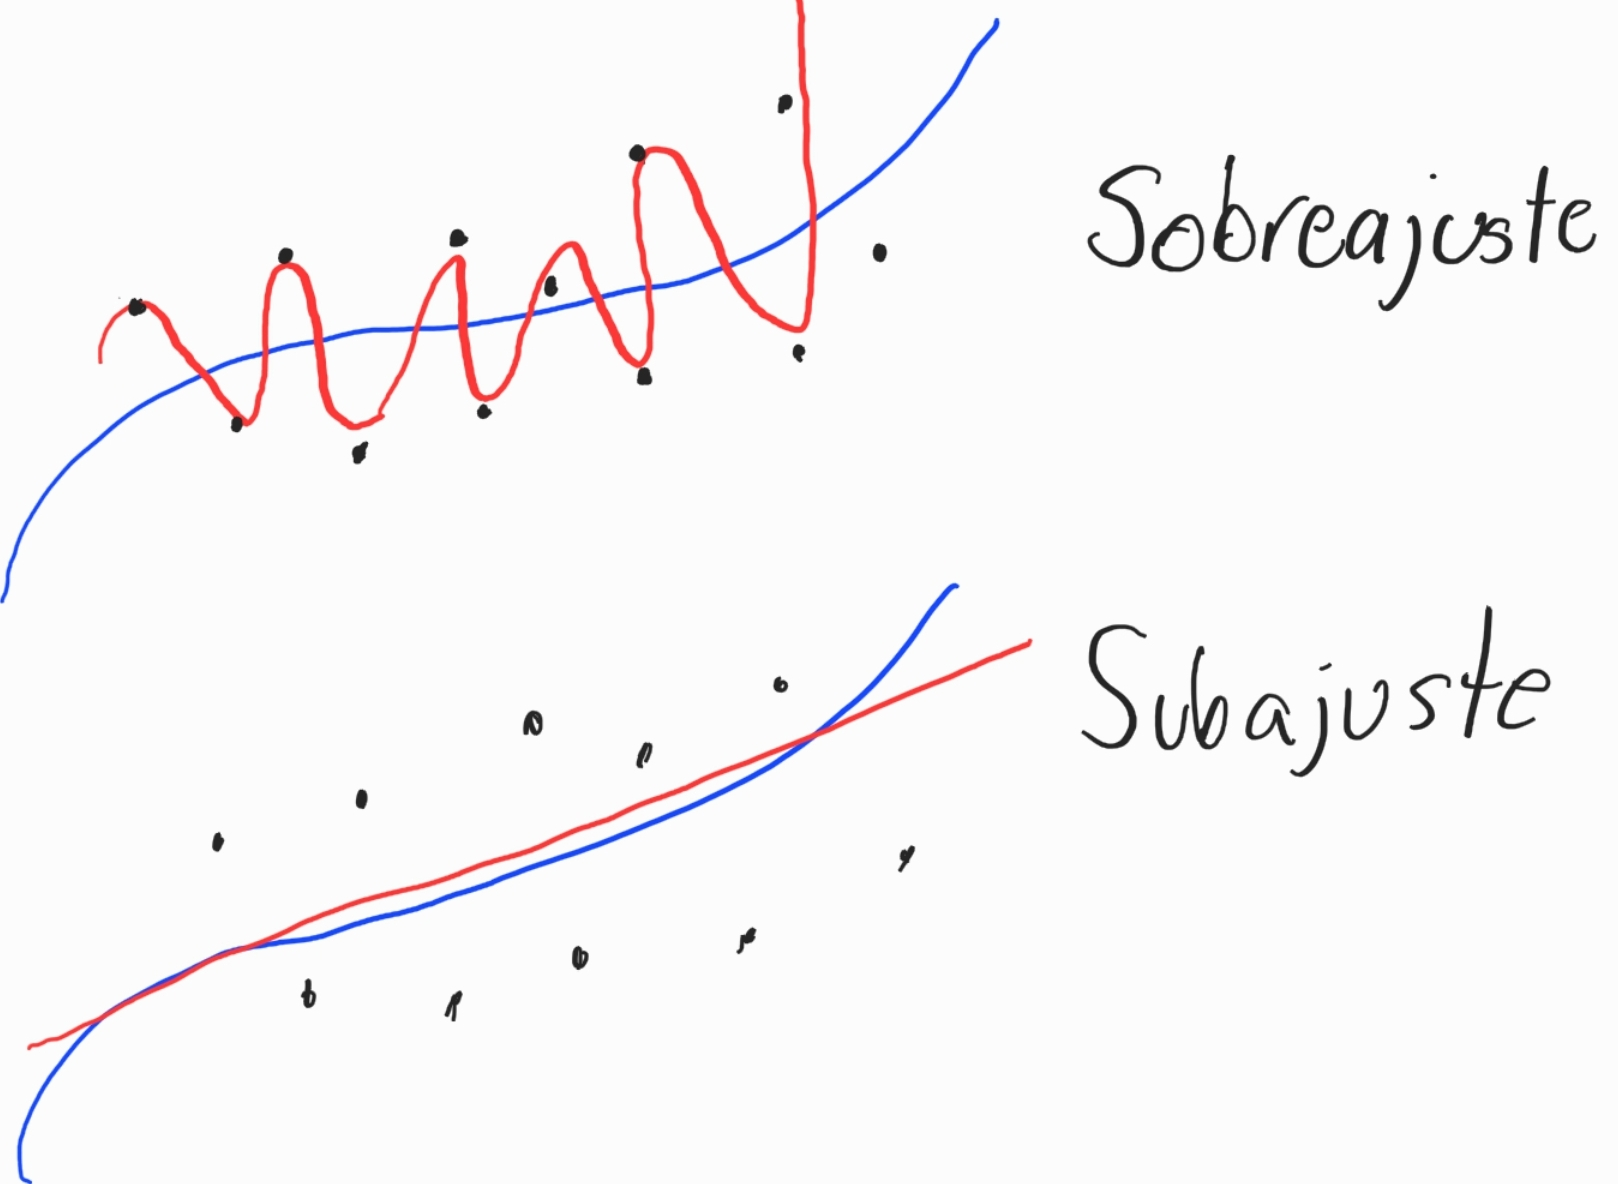
\includegraphics[width=0.6\columnwidth]{Ej_Flex_Fam.jpg}
      \caption{{\textsf{Ejemplo de modelos con familias sobreajustadas y subajustadas.}}  }\label{fig:bell-curve}
    \end{figure}

\end{document}
